\documentclass[12pt,a4paper]{article}
\usepackage[utf8]{vietnam}
\usepackage{amsmath,amssymb,amsfonts,mathrsfs}
\usepackage[left=1.5cm,right=1.5cm,top=2cm,bottom=2cm,headheight=17pt]{geometry}
\usepackage{enumitem}
\usepackage{array}
\usepackage{graphicx}
\usepackage{tikz}
\usetikzlibrary{arrows.meta,calc,patterns}
\usepackage{fancyhdr}

\pagestyle{fancy}
\fancyhf{}
\lhead{\small\textbf{HƯỚNG TỚI THPTQG 2027}}
\rhead{\small\textit{Người biên soạn: Dương Gia Bảo}}
\rfoot{\small Trang \thepage}
\renewcommand{\headrulewidth}{0.4pt}

\begin{document}

\noindent
\begin{minipage}[t]{0.40\textwidth}
    \centering
    \textbf{HƯỚNG TỚI THPTQG 2027}\\[-2pt]
    \rule{3.2cm}{0.6pt}\\[4pt]
    \textbf{ĐỀ CHÍNH THỨC}
\end{minipage}\hfill
\begin{minipage}[t]{0.58\textwidth}
    \centering
    \textbf{ĐỀ THI KHẢO SÁT CHẤT LƯỢNG}\\
    \textbf{ĐỀ SỐ 11}\\
    \textbf{Môn thi: TOÁN}\\
    \textit{\small Thời gian làm bài: 90 phút, không kể thời gian phát đề}
\end{minipage}

\vspace{0.2cm}
\noindent
\begin{minipage}[b]{0.78\textwidth}
    \textbf{Họ và tên:}\dotfill\textbf{SBD:}\makebox[3.5cm]{\dotfill}
\end{minipage}\hfill
\begin{minipage}[b]{0.20\textwidth}
    \hfill
    \setlength{\fboxrule}{0.8pt}%
    \fbox{\begin{minipage}{2.3cm}
        \centering
        \textbf{\small Mã đề thi}\\
        \textbf{0011}
    \end{minipage}}
\end{minipage}
\vspace{0.2cm}

% ==========================================
% PHẦN I
% ==========================================
\section*{\large PHẦN I. CÂU TRẮC NGHIỆM NHIỀU PHƯƠNG ÁN LỰA CHỌN}
\textit{Thí sinh trả lời từ câu 1 đến câu 12. Mỗi câu hỏi thí sinh chỉ chọn một phương án. Mỗi câu trả lời đúng được 0,25 điểm.}

\begin{enumerate}[label=\textbf{Câu \arabic*:}, leftmargin=*]

\item Cho hàm số $y = \dfrac{x^2 + 2x - 2}{x - 1}$ có đồ thị $(C)$. Tâm đối xứng của đồ thị $(C)$ là điểm
\begin{enumerate}[label=\Alph*.]
    \item $I(1; 4)$.
    \item $I(-1; 4)$.
    \item $I(1; 2)$.
    \item $I(0; 2)$.
\end{enumerate}

\item Tập nghiệm $S$ của bất phương trình $\log_3(2x - 1) \le 2$ là
\begin{enumerate}[label=\Alph*.]
    \item $S = (0; 5]$.
    \item $S = [1; 5]$.
    \item $S = \left(\dfrac{1}{2}; 5\right]$.
    \item $S = (-\infty; 5]$.
\end{enumerate}

\item Họ tất cả các nguyên hàm của hàm số $f(x) = e^{3x}$ là
\begin{enumerate}[label=\Alph*.]
    \item $F(x) = 3e^{3x} + C$.
    \item $F(x) = \dfrac{1}{3}e^{3x} + C$.
    \item $F(x) = e^{3x} + C$.
    \item $F(x) = \dfrac{1}{3}e^x + C$.
\end{enumerate}

\item Trong không gian $Oxyz$, mặt phẳng đi qua điểm $M(1; -2; 3)$ và nhận vectơ $\vec{n} = (2; -1; 4)$ làm vectơ pháp tuyến có phương trình là
\begin{enumerate}[label=\Alph*.]
    \item $2x - y + 4z + 16 = 0$.
    \item $2x - y + 4z = 0$.
    \item $x - 2y + 3z - 16 = 0$.
    \item $2x - y + 4z - 16 = 0$.
\end{enumerate}

\item Hai xạ thủ độc lập cùng bắn vào một mục tiêu, mỗi người bắn đúng một phát. Xác suất bắn trúng của xạ thủ thứ nhất là $0{,}7$ và của xạ thủ thứ hai là $0{,}8$. Xác suất để có đúng một xạ thủ bắn trúng mục tiêu bằng
\begin{enumerate}[label=\Alph*.]
    \item $0{,}56$.
    \item $0{,}38$.
    \item $0{,}44$.
    \item $0{,}26$.
\end{enumerate}

\item Thời gian hoàn thành một sản phẩm thủ công (đơn vị: ngày) của $40$ nghệ nhân được ghi nhận trong bảng số liệu ghép nhóm sau:
\begin{center}
\begin{tabular}{|c|c|c|c|c|c|}
\hline
\textbf{Thời gian (ngày)} & $[4; 5)$ & $[5; 6)$ & $[6; 7)$ & $[7; 8)$ & $[8; 9)$ \\ \hline
\textbf{Số nghệ nhân} & 3 & 7 & 12 & 14 & 4 \\ \hline
\end{tabular}
\end{center}
Khoảng biến thiên $R$ của mẫu số liệu ghép nhóm trên bằng
\begin{enumerate}[label=\Alph*.]
    \item $R = 5$.
    \item $R = 4$.
    \item $R = 6$.
    \item $R = 9$.
\end{enumerate}

\item Cho hình chóp $S.ABC$ có cạnh bên $SA$ vuông góc với mặt phẳng đáy $(ABC)$. Đáy $ABC$ là tam giác vuông tại $B$ với $AB = a$, cạnh bên $SA = a\sqrt{3}$. Khoảng cách từ điểm $A$ đến mặt phẳng $(SBC)$ bằng
\begin{enumerate}[label=\Alph*.]
    \item $\dfrac{a}{2}$.
    \item $a\sqrt{3}$.
    \item $a$.
    \item $\dfrac{a\sqrt{3}}{2}$.
\end{enumerate}

\item Cho cấp số cộng $(u_n)$ có số hạng đầu $u_1 = 3$ và công sai $d = 4$. Số hạng thứ mười $u_{10}$ của cấp số cộng bằng
\begin{enumerate}[label=\Alph*.]
    \item $43$.
    \item $36$.
    \item $39$.
    \item $40$.
\end{enumerate}

\item Khối lượng của một chất phóng xạ phân rã sau $t$ ngày được xác định bởi công thức $m(t) = m_0 \cdot 2^{-t/T}$, trong đó $m_0$ là khối lượng ban đầu và $T$ là chu kỳ bán rã. Biết ban đầu mẫu có khối lượng $m_0 = 100\text{ g}$ và chu kỳ bán rã $T = 8$ ngày. Sau $24$ ngày, khối lượng chất phóng xạ còn lại trong mẫu bằng
\begin{enumerate}[label=\Alph*.]
    \item $25\text{ g}$.
    \item $12{,}5\text{ g}$.
    \item $6{,}25\text{ g}$.
    \item $50\text{ g}$.
\end{enumerate}

\item Trong không gian $Oxyz$, cho hai điểm $A(1; 0; -1)$ và $B(2; -1; 1)$. Phương trình chính tắc của đường thẳng $AB$ là
\begin{enumerate}[label=\Alph*.]
    \item $\dfrac{x + 1}{1} = \dfrac{y}{-1} = \dfrac{z - 1}{2}$.
    \item $\dfrac{x - 1}{1} = \dfrac{y}{1} = \dfrac{z + 1}{2}$.
    \item $\dfrac{x - 2}{1} = \dfrac{y + 1}{-1} = \dfrac{z - 1}{-2}$.
    \item $\dfrac{x - 1}{1} = \dfrac{y}{-1} = \dfrac{z + 1}{2}$.
\end{enumerate}

\item Một người thợ dùng một đoạn dây thép dài $20\text{ m}$ để uốn thành khung một luống hoa hình chữ nhật. Diện tích lớn nhất của luống hoa có thể tạo thành bằng bao nhiêu mét vuông?
\begin{enumerate}[label=\Alph*.]
    \item $25\text{ m}^2$.
    \item $20\text{ m}^2$.
    \item $16\text{ m}^2$.
    \item $36\text{ m}^2$.
\end{enumerate}

\item Cho hình nón có bán kính đáy $R = 3a$ và chiều cao $h = 4a$. Thể tích của khối nón tròn xoay đã cho bằng
\begin{enumerate}[label=\Alph*.]
    \item $36\pi a^3$.
    \item $15\pi a^3$.
    \item $12\pi a^3$.
    \item $4\pi a^3$.
\end{enumerate}

\end{enumerate}

% ==========================================
% PHẦN II
% ==========================================
\vspace{0.4cm}
\section*{\large PHẦN II. CÂU TRẮC NGHIỆM ĐÚNG SAI}
\textit{Thí sinh trả lời từ câu 1 đến câu 4. Trong mỗi ý \textbf{a)}, \textbf{b)}, \textbf{c)}, \textbf{d)} ở mỗi câu, thí sinh chọn đúng hoặc sai.}

\begin{enumerate}[label=\textbf{Câu \arabic*:}, leftmargin=*]

\item Cho hàm số $y = \dfrac{2x^2 - 3x + 3}{x - 1}$ có đồ thị $(C)$.
\begin{enumerate}[label=\textbf{\alph*)}]
    \item Hàm số đạt cực đại tại $x = 0$ và đạt cực tiểu tại $x = 2$.
    \item Đường thẳng đi qua hai điểm cực trị của đồ thị $(C)$ có phương trình $y = 4x - 3$.
    \item Giao điểm của hai đường tiệm cận của đồ thị $(C)$ là điểm $I(1; 2)$.
    \item Tiếp tuyến của đồ thị $(C)$ tại điểm có hoành độ $x = 3$ có hệ số góc bằng $\dfrac{3}{2}$.
\end{enumerate}

\item Chi phí nhiên liệu vận hành của một chiếc tàu thủy khi di chuyển trên sông gồm hai phần: phần thứ nhất cố định bằng $720$ nghìn đồng/giờ; phần thứ hai tỉ lệ thuận với bình phương vận tốc của tàu, khi tàu chạy với vận tốc $v = 10\text{ km/h}$ thì phần thứ hai bằng $80$ nghìn đồng/giờ.
\begin{enumerate}[label=\textbf{\alph*)}]
    \item Hàm số xác định tổng chi phí nhiên liệu cho mỗi ki-lô-mét đường sông khi tàu chạy với vận tốc $v$ (km/h) là $f(v) = \dfrac{720}{v} + 0{,}8v$ (nghìn đồng).
    \item Khi tàu chạy với vận tốc $v = 10\text{ km/h}$, chi phí nhiên liệu trên mỗi ki-lô-mét đường sông bằng $72$ nghìn đồng.
    \item Vận tốc của tàu để tổng chi phí nhiên liệu trên mỗi ki-lô-mét đường sông đạt giá trị nhỏ nhất là $v = 30\text{ km/h}$.
    \item Chi phí nhiên liệu nhỏ nhất trên mỗi ki-lô-mét đường sông bằng $48$ nghìn đồng.
\end{enumerate}

\item \begin{minipage}[t]{0.55\linewidth}
Một giàn đèn sân khấu có trọng lượng $P = 540\text{ N}$ được treo cố định tại điểm $S(0; 0; 0)$ trong không gian $Oxyz$ (đơn vị đo trên các trục là mét). Trần nhà là mặt phẳng có phương trình $z = 3$. Giàn đèn được giữ cân bằng bởi ba sợi dây cáp căng nối từ $S$ đến ba điểm cố định trên trần nhà là $A(0; 4; 3)$, $B(-2\sqrt{3}; -2; 3)$ và $C(2\sqrt{3}; -2; 3)$. Trọng lực tác dụng lên giàn đèn có vectơ $\vec{P} = (0; 0; -540)$.
\begin{enumerate}[label=\textbf{\alph*)}]
    \item Chiều dài của mỗi sợi dây cáp treo bằng $5\text{ m}$.
    \item Cosin của góc giữa mỗi sợi dây cáp và trần nhà bằng $\dfrac{4}{5}$.
    \item Cosin của góc tạo bởi hai sợi dây cáp $SA$ và $SB$ bằng $\dfrac{1}{5}$.
    \item Lực căng tác dụng lên mỗi sợi dây cáp có độ lớn bằng $300\text{ N}$.
\end{enumerate}
\end{minipage}\hfill
\begin{minipage}[t]{0.42\linewidth}
\vspace{-0.4\baselineskip}
\centering
\resizebox{\linewidth}{!}{%
\begin{tikzpicture}[>=Stealth, line join=round, line cap=round, scale=0.9]
    % Mặt phẳng trần nhà z = 3 nhìn xiên thoáng đãng
    \draw[dashed, thin, fill=gray!8, fill opacity=0.5] 
        (-3.2,1.2) -- (3.2,1.2) -- (4.2,4.2) -- (-2.2,4.2) -- cycle;
    \node[right, font=\footnotesize, text=gray!80!black] at (4.0,4.0) {Trần ($z=3$)};

    % Tọa độ các điểm neo trên trần nhà
    \coordinate (A) at (0,3.6);
    \coordinate (B) at (-1.8,1.8);
    \coordinate (C) at (2.2,2.0);
    \coordinate (S) at (0.2,-0.8);

    % Tam giác đáy neo ABC trên trần
    \draw[dashed, thin, gray!70] (A) -- (B) -- (C) -- cycle;

    % Ba sợi dây cáp SA, SB, SC
    \draw[very thick, blue!65!black] (S) -- (A);
    \draw[very thick, blue!65!black] (S) -- (B);
    \draw[very thick, blue!65!black] (S) -- (C);

    % Vectơ trọng lực P chỉ thẳng đứng xuống dưới
    \draw[->, very thick, red!85!black] (S) -- ($(S) + (0,-1.6)$) node[right, font=\small] {$\vec{P}$};

    % Các điểm mốc
    \filldraw (A) circle (2pt) node[above, fill=white, inner sep=1pt] {$A$};
    \filldraw (B) circle (2pt) node[below left, fill=white, inner sep=1pt] {$B$};
    \filldraw (C) circle (2pt) node[right, fill=white, inner sep=1pt] {$C$};
    \filldraw[fill=orange!85!yellow, draw=black, thick] (S) circle (2.8pt) node[left, fill=white, inner sep=1pt] {$S$};
\end{tikzpicture}%
}
\end{minipage}

\item Khảo sát điểm thi thử tốt nghiệp THPT môn Toán của $40$ học sinh lớp 12A1 và $40$ học sinh lớp 12A2, người ta thu được bảng phân bố tần số ghép nhóm sau:
\begin{center}
\begin{tabular}{|c|c|c|c|c|}
\hline
\textbf{Điểm số} & $[6; 7)$ & $[7; 8)$ & $[8; 9)$ & $[9; 10)$ \\ \hline
\textbf{Số học sinh lớp 12A1} & 4 & 16 & 16 & 4 \\ \hline
\textbf{Số học sinh lớp 12A2} & 8 & 12 & 12 & 8 \\ \hline
\end{tabular}
\end{center}
\begin{enumerate}[label=\textbf{\alph*)}]
    \item Điểm trung bình môn Toán của học sinh lớp 12A1 bằng $8{,}0$.
    \item Phương sai của điểm thi học sinh lớp 12A1 bằng $0{,}85$.
    \item Độ lệch chuẩn điểm thi của học sinh lớp 12A1 nhỏ hơn độ lệch chuẩn điểm thi của học sinh lớp 12A2.
    \item Kết quả điểm thi của học sinh lớp 12A1 có mức độ đồng đều cao hơn học sinh lớp 12A2.
\end{enumerate}

\end{enumerate}

% ==========================================
% PHẦN III
% ==========================================
\vspace{0.4cm}
\section*{\large PHẦN III. CÂU TRẮC NGHIỆM TRẢ LỜI NGẮN}
\textit{Thí sinh trả lời từ câu 1 đến câu 6. Mỗi câu trả lời đúng được 0,5 điểm.}

\begin{enumerate}[label=\textbf{Câu \arabic*:}, leftmargin=*]

\item Một thùng đựng sơn hình trụ có bán kính đáy $R = \dfrac{6}{\pi}\text{ cm}$ và chiều cao $h = 8\text{ cm}$. Một chú kiến bò trên bề mặt bên ngoài của thùng từ một điểm $A$ ở vành đáy dưới đến điểm $B$ ở vành đáy trên nằm đối diện với điểm $A$ qua trục hình trụ (cách $A$ nửa vòng tròn theo đường biên đáy). Quãng đường ngắn nhất mà chú kiến cần bò bằng bao nhiêu xăng-ti-mét?

\item \begin{minipage}[t]{0.55\linewidth}
Một cửa hầm đường bộ có mặt cắt là hình phẳng được giới hạn bởi một parabol và mặt đất nằm ngang. Chọn hệ trục tọa độ sao cho mặt đất nằm trên trục hoành $Ox$, đường parabol có phương trình $y = 12 - 3x^2$ (đơn vị trên các trục là mét, với $-2 \le x \le 2$). Để gia cố kết cấu hầm, người ta đặt một thanh dầm ngang tại độ cao $y = 9$. Phần diện tích vòm hầm phía trên thanh dầm (phần gạch chéo trong hình vẽ) được ốp tấm thép chịu lực. Diện tích phần vòm hầm được ốp tấm thép chịu lực bằng bao nhiêu mét vuông?
\end{minipage}\hfill
\begin{minipage}[t]{0.42\linewidth}
\vspace{-0.4\baselineskip}
\centering
\resizebox{\linewidth}{!}{%
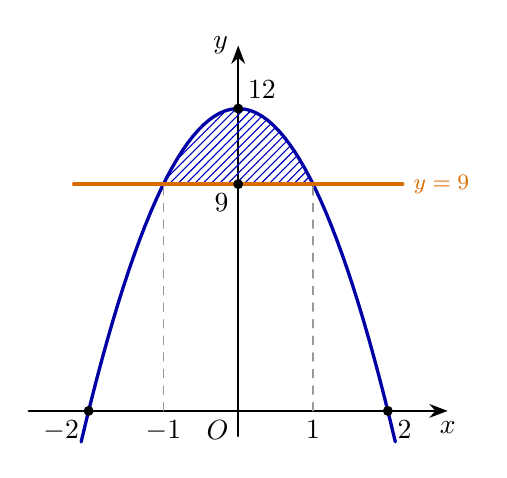
\begin{tikzpicture}[>=Stealth, x=0.95cm, y=0.32cm, line join=round, line cap=round]
    % Trục tọa độ
    \draw[->, thick] (-2.8,0) -- (2.8,0) node[below] {$x$};
    \draw[->, thick] (0,-1) -- (0,14.5) node[left] {$y$};
    \node[below left] at (0,0) {$O$};

    % Miền gạch chéo phía trên thanh dầm y = 9 từ x = -1 đến 1
    \fill[pattern=north east lines, pattern color=blue!75!black, domain=-1:1, samples=40] 
        plot (\x, {12 - 3*(\x)^2}) -- (-1,9) -- cycle;

    % Đường parabol và thanh dầm
    \draw[very thick, blue!65!black, domain=-2.1:2.1, samples=60] plot (\x, {12 - 3*(\x)^2});
    \draw[very thick, orange!85!black] (-2.2,9) -- (2.2,9) node[right, font=\footnotesize] {$y = 9$};

    % Hai đường dóng xuống trục hoành
    \draw[dashed, thin, gray!80] (-1,0) -- (-1,9);
    \draw[dashed, thin, gray!80] (1,0) -- (1,9);

    % Tọa độ các mốc
    \node[below] at (-1,0) {$-1$};
    \node[below] at (1,0) {$1$};
    \fill (0,12) circle (1.8pt) node[above right] {$12$};
    \fill (0,9) circle (1.8pt) node[below left] {$9$};
    \fill (-2,0) circle (1.8pt) node[below left] {$-2$};
    \fill (2,0) circle (1.8pt) node[below right] {$2$};
\end{tikzpicture}%
}
\end{minipage}

\item Một tấm bảng áp phích quảng cáo có chiều cao $AB = 3\text{ m}$ được treo thẳng đứng trên một bức tường, mép dưới $A$ của bảng cách mặt đất $1\text{ m}$ (mép trên $B$ cách mặt đất $4\text{ m}$). Một ống kính quan sát đặt tại điểm $C$ trên mặt đất cách chân tường một khoảng $x$ (mét) ($x > 0$). Để góc quan sát tấm bảng $\widehat{ACB}$ đạt giá trị lớn nhất thì ống kính phải đặt cách chân tường một khoảng bằng bao nhiêu mét?

\item Trong không gian $Oxyz$, cho mặt phẳng $(P): 2x - 2y + z + 12 = 0$ và điểm $A(1; 3; -2)$. Một thiết bị bay thám hiểm di chuyển trên mặt phẳng $(P)$. Khoảng cách ngắn nhất từ điểm $A$ đến thiết bị bay bằng bao nhiêu?

\item \begin{minipage}[t]{0.65\linewidth}
Trong một đợt thi đấu giải vô địch, siêu sao bóng đá Cristiano Ronaldo thực hiện một loạt gồm $5$ quả sút luân lưu $11\text{m}$. Giả sử các lần sút là hoàn toàn độc lập với nhau và xác suất thực hiện thành công ở mỗi lần sút của anh đều bằng $0{,}9$. Xác suất để Cristiano Ronaldo sút thành công cả $5$ quả luân lưu bằng bao nhiêu? (kết quả làm tròn đến hàng phần trăm).
\end{minipage}\hfill
\begin{minipage}[t]{0.32\linewidth}
\vspace{-0.5\baselineskip}
\centering

\includegraphics[width=\linewidth, keepaspectratio]{cr7_football.png}
\end{minipage}

\item Một chi tiết linh kiện máy móc nằm giữa hai mặt phẳng $x = 0$ và $x = 3$. Cắt chi tiết máy bởi mặt phẳng vuông góc với trục $Ox$ tại điểm có hoành độ $x$ ($0 \le x \le 3$), thiết diện thu được là một hình vuông có độ dài cạnh bằng $\sqrt{3x^2 + 1}$ (đơn vị: dm). Thể tích của chi tiết máy đó bằng bao nhiêu đề-xi-mét khối?

\end{enumerate}

% ==========================================
% BẢNG ĐÁP ÁN TỔNG HỢP (BẮT BUỘC TRANG MỚI)
% ==========================================
\newpage
\begin{center}
    {\Large\textbf{BẢNG ĐÁP ÁN TỔNG HỢP}}\\[4pt]
    \textbf{ĐỀ SỐ 11 - MÔN: TOÁN}
\end{center}
\vspace{0.3cm}

\noindent\textbf{\large PHẦN I. CÂU TRẮC NGHIỆM NHIỀU PHƯƠNG ÁN LỰA CHỌN}
\begin{center}
\renewcommand{\arraystretch}{1.25}
\begin{tabular}{|c|c|c|c|c|c|c|c|c|c|c|c|}
\hline
\textbf{1} & \textbf{2} & \textbf{3} & \textbf{4} & \textbf{5} & \textbf{6} & \textbf{7} & \textbf{8} & \textbf{9} & \textbf{10} & \textbf{11} & \textbf{12} \\ \hline
\textbf{A} & \textbf{C} & \textbf{B} & \textbf{D} & \textbf{B} & \textbf{A} & \textbf{D} & \textbf{C} & \textbf{B} & \textbf{D} & \textbf{A} & \textbf{C} \\ \hline
\end{tabular}
\end{center}

\vspace{0.3cm}
\noindent\textbf{\large PHẦN II. CÂU TRẮC NGHIỆM ĐÚNG SAI}
\begin{center}
\renewcommand{\arraystretch}{1.25}
\begin{tabular}{|c|c|c|c|c|}
\hline
\textbf{Câu} & \textbf{Ý a)} & \textbf{Ý b)} & \textbf{Ý c)} & \textbf{Ý d)} \\ \hline
\textbf{Câu 1} & Đ & Đ & S & Đ \\ \hline
\textbf{Câu 2} & Đ & S & Đ & Đ \\ \hline
\textbf{Câu 3} & Đ & Đ & S & Đ \\ \hline
\textbf{Câu 4} & Đ & S & Đ & Đ \\ \hline
\end{tabular}
\end{center}

\vspace{0.3cm}
\noindent\textbf{\large PHẦN III. CÂU TRẮC NGHIỆM TRẢ LỜI NGẮN}
\begin{center}
\renewcommand{\arraystretch}{1.25}
\begin{tabular}{|c|c|c|c|c|c|}
\hline
\textbf{Câu 1} & \textbf{Câu 2} & \textbf{Câu 3} & \textbf{Câu 4} & \textbf{Câu 5} & \textbf{Câu 6} \\ \hline
10 & 4 & 2 & 2 & 0,59 & 30 \\ \hline
\end{tabular}
\end{center}

% ==========================================
% HƯỚNG DẪN GIẢI CHI TIẾT
% ==========================================
\newpage
\begin{center}
    {\Large\textbf{HƯỚNG DẪN GIẢI CHI TIẾT}}\\[4pt]
    \textbf{ĐỀ SỐ 11 - MÔN: TOÁN}
\end{center}
\vspace{0.3cm}

\section*{\large PHẦN I. CÂU TRẮC NGHIỆM NHIỀU PHƯƠNG ÁN LỰA CHỌN}

\noindent\textbf{Câu 1.} Thực hiện phép chia đa thức tử cho mẫu:
\[
\dfrac{x^2 + 2x - 2}{x - 1} = x + 3 + \dfrac{1}{x - 1}.
\]
Đường tiệm cận đứng là $x = 1$. Đường tiệm cận xiên là $y = x + 3$.\\
Tâm đối xứng $I$ của đồ thị là giao điểm của hai đường tiệm cận:
\[
\begin{cases}
x = 1 \\
y = x + 3
\end{cases}
\implies I(1; 4).
\]
\textbf{Chọn A.}

\vspace{0.25cm}
\noindent\textbf{Câu 2.} Điều kiện xác định: $2x - 1 > 0 \iff x > \dfrac{1}{2}$.\\
Bất phương trình đã cho tương đương với:
\[
2x - 1 \le 3^2 \iff 2x - 1 \le 9 \iff 2x \le 10 \iff x \le 5.
\]
Kết hợp với điều kiện xác định, ta được tập nghiệm $S = \left(\dfrac{1}{2}; 5\right]$.\\
\textbf{Chọn C.}

\vspace{0.25cm}
\noindent\textbf{Câu 3.} Ta có công thức nguyên hàm cơ bản:
\[
\int e^{ax+b}\,\text{d}x = \dfrac{1}{a}e^{ax+b} + C.
\]
Do đó: $\int e^{3x}\,\text{d}x = \dfrac{1}{3}e^{3x} + C$.\\
\textbf{Chọn B.}

\vspace{0.25cm}
\noindent\textbf{Câu 4.} Phương trình mặt phẳng đi qua $M(x_0; y_0; z_0)$ nhận $\vec{n} = (A; B; C)$ làm VTPT là:
\[
A(x - x_0) + B(y - y_0) + C(z - z_0) = 0.
\]
Với $M(1; -2; 3)$ và $\vec{n} = (2; -1; 4)$, ta có:
\[
2(x - 1) - 1(y + 2) + 4(z - 3) = 0 \iff 2x - y + 4z - 16 = 0.
\]
\textbf{Chọn D.}

\vspace{0.25cm}
\noindent\textbf{Câu 5.} Gọi $A$ là biến cố "Xạ thủ thứ nhất bắn trúng", $B$ là biến cố "Xạ thủ thứ hai bắn trúng".\\
Theo giả thiết: $P(A) = 0{,}7 \implies P(\overline{A}) = 0{,}3$; $P(B) = 0{,}8 \implies P(\overline{B}) = 0{,}2$.\\
Biến cố có đúng một người bắn trúng mục tiêu là $C = (A \cap \overline{B}) \cup (\overline{A} \cap B)$.\\
Do $A$ và $B$ độc lập nên:
\[
P(C) = P(A) \cdot P(\overline{B}) + P(\overline{A}) \cdot P(B) = 0{,}7 \cdot 0{,}2 + 0{,}3 \cdot 0{,}8 = 0{,}14 + 0{,}24 = 0{,}38.
\]
\textbf{Chọn B.}

\vspace{0.25cm}
\noindent\textbf{Câu 6.} Khoảng biến thiên của mẫu số liệu ghép nhóm là hiệu giữa đầu mút phải của nhóm cuối cùng và đầu mút trái của nhóm đầu tiên:
\[
R = 9 - 4 = 5.
\]
\textbf{Chọn A.}

\vspace{0.25cm}
\noindent\textbf{Câu 7.} Ta có $SA \perp (ABC) \implies SA \perp BC$.\\
Mặt khác đáy $ABC$ vuông tại $B$ nên $AB \perp BC$.\\
Suy ra $BC \perp (SAB)$, dẫn đến $(SBC) \perp (SAB)$ theo giao tuyến $SB$.\\
Trong mặt phẳng $(SAB)$, kẻ đường cao $AH \perp SB$ ($H \in SB$). Do $(SBC) \perp (SAB)$ nên $AH \perp (SBC)$.\\
Khoảng cách từ $A$ đến mặt phẳng $(SBC)$ bằng độ dài $AH$.\\
Áp dụng hệ thức lượng trong tam giác vuông $SAB$ tại $A$:
\[
AH = \dfrac{SA \cdot AB}{\sqrt{SA^2 + AB^2}} = \dfrac{a\sqrt{3} \cdot a}{\sqrt{3a^2 + a^2}} = \dfrac{a\sqrt{3}}{2}.
\]
\textbf{Chọn D.}

\vspace{0.25cm}
\noindent\textbf{Câu 8.} Số hạng tổng quát của cấp số cộng là $u_n = u_1 + (n - 1)d$.\\
Với $n = 10$, ta có:
\[
u_{10} = u_1 + 9d = 3 + 9 \cdot 4 = 3 + 36 = 39.
\]
\textbf{Chọn C.}

\vspace{0.25cm}
\noindent\textbf{Câu 9.} Thay $m_0 = 100\text{ g}$, $T = 8$ ngày và $t = 24$ ngày vào công thức:
\[
m(24) = 100 \cdot 2^{-24/8} = 100 \cdot 2^{-3} = 100 \cdot \dfrac{1}{8} = 12{,}5\text{ g}.
\]
\textbf{Chọn B.}

\vspace{0.25cm}
\noindent\textbf{Câu 10.} Vectơ chỉ phương của đường thẳng $AB$ là:
\[
\vec{AB} = (2 - 1;\ -1 - 0;\ 1 - (-1)) = (1; -1; 2).
\]
Đường thẳng $AB$ đi qua điểm $A(1; 0; -1)$ có phương trình chính tắc:
\[
\dfrac{x - 1}{1} = \dfrac{y}{-1} = \dfrac{z + 1}{2}.
\]
\textbf{Chọn D.}

\vspace{0.25cm}
\noindent\textbf{Câu 11.} Gọi chiều dài và chiều rộng của luống hoa là $x$ và $y$ ($0 < x, y < 10$, tính theo mét).\\
Chu vi luống hoa bằng $2(x + y) = 20 \implies x + y = 10 \implies y = 10 - x$.\\
Diện tích của luống hoa là:
\[
S(x) = x(10 - x) = -x^2 + 10x.
\]
Hàm $S(x)$ đạt giá trị lớn nhất tại đỉnh parabol $x = -\dfrac{10}{2(-1)} = 5$.\\
Diện tích lớn nhất là $S_{\max} = 5(10 - 5) = 25\text{ m}^2$.\\
\textbf{Chọn A.}

\vspace{0.25cm}
\noindent\textbf{Câu 12.} Thể tích của khối nón tròn xoay là:
\[
V = \dfrac{1}{3}\pi R^2 h = \dfrac{1}{3}\pi (3a)^2 (4a) = \dfrac{1}{3}\pi \cdot 9a^2 \cdot 4a = 12\pi a^3.
\]
\textbf{Chọn C.}

% ==========================================
\vspace{0.4cm}
\section*{\large PHẦN II. CÂU TRẮC NGHIỆM ĐÚNG SAI}

\noindent\textbf{Câu 1.}
Tập xác định: $D = \mathbb{R} \setminus \{1\}$. Ta có $y = \dfrac{2x^2 - 3x + 3}{x - 1} = 2x - 1 + \dfrac{2}{x - 1}$.\\
Đạo hàm:
\[
y' = 2 - \dfrac{2}{(x - 1)^2} = \dfrac{2(x - 1)^2 - 2}{(x - 1)^2} = \dfrac{2(x^2 - 2x)}{(x - 1)^2}.
\]
Cho $y' = 0 \iff x = 0$ hoặc $x = 2$.\\
Bảng biến thiên:
\begin{itemize}
    \item Trên $(-\infty; 0)$ và $(2; +\infty)$: $y' > 0$, hàm số đồng biến.
    \item Trên $(0; 1)$ và $(1; 2)$: $y' < 0$, hàm số nghịch biến.
\end{itemize}
Hàm số đạt cực đại tại $x = 0$ với $y(0) = -3$; đạt cực tiểu tại $x = 2$ với $y(2) = 5$.\\
$\implies$ \textbf{a) ĐÚNG.}

Đường thẳng đi qua hai điểm cực trị của hàm phân thức bậc hai trên bậc nhất $y = \dfrac{u(x)}{v(x)}$ có phương trình là $y = \dfrac{u'(x)}{v'(x)} = \dfrac{4x - 3}{1} = 4x - 3$.\\
Kiểm tra: tại cực đại $(0; -3)$, $-3 = 4(0) - 3$; tại cực tiểu $(2; 5)$, $5 = 4(2) - 3$ (thỏa mãn).\\
$\implies$ \textbf{b) ĐÚNG.}

Đường tiệm cận đứng là $x = 1$. Đường tiệm cận xiên là $y = 2x - 1$.\\
Giao điểm $I$ của hai đường tiệm cận có tọa độ là nghiệm hệ $\begin{cases} x = 1 \\ y = 2(1) - 1 = 1 \end{cases} \implies I(1; 1) \ne (1; 2)$.\\
$\implies$ \textbf{c) SAI.}

Tại điểm có hoành độ $x = 3$, hệ số góc của tiếp tuyến là:
\[
k = y'(3) = 2 - \dfrac{2}{(3 - 1)^2} = 2 - \dfrac{2}{4} = 2 - \dfrac{1}{2} = \dfrac{3}{2}.
\]
$\implies$ \textbf{d) ĐÚNG.}

\vspace{0.3cm}
\noindent\textbf{Câu 2.}
Phần chi phí thứ nhất cố định là $C_1 = 720$ nghìn đồng/giờ.\\
Phần chi phí thứ hai tỉ lệ thuận với $v^2$, có dạng $C_2(v) = k v^2$.\\
Khi $v = 10\text{ km/h}$ thì $C_2(10) = k \cdot 100 = 80 \implies k = 0{,}8$ (nghìn đồng/(km/h)$^2$).\\
Do đó, tổng chi phí nhiên liệu trong $1$ giờ là $C(v) = 720 + 0{,}8v^2$ (nghìn đồng/giờ).\\
Để đi được $1\text{ km}$, thời gian tàu cần chạy là $t = \dfrac{1}{v}$ giờ.\\
Tổng chi phí nhiên liệu trên mỗi ki-lô-mét đường sông là:
\[
f(v) = C(v) \cdot t = \dfrac{720 + 0{,}8v^2}{v} = \dfrac{720}{v} + 0{,}8v\text{ (nghìn đồng)}.
\]
$\implies$ \textbf{a) ĐÚNG.}

Khi tàu chạy với vận tốc $v = 10\text{ km/h}$, chi phí nhiên liệu trên $1\text{ km}$ là:
\[
f(10) = \dfrac{720}{10} + 0{,}8(10) = 72 + 8 = 80\text{ (nghìn đồng)} \ne 72\text{ nghìn đồng}.
\]
$\implies$ \textbf{b) SAI.}

Xét hàm số $f(v) = \dfrac{720}{v} + 0{,}8v$ với $v > 0$:\\
Đạo hàm: $f'(v) = -\dfrac{720}{v^2} + 0{,}8$. Cho $f'(v) = 0 \iff v^2 = \dfrac{720}{0{,}8} = 900 \iff v = 30\text{ km/h}$.\\
Bảng biến thiên cho thấy $f(v)$ đạt giá trị nhỏ nhất tại $v = 30\text{ km/h}$.\\
$\implies$ \textbf{c) ĐÚNG.}

Chi phí nhiên liệu nhỏ nhất trên mỗi ki-lô-mét đường sông là:
\[
f(30) = \dfrac{720}{30} + 0{,}8(30) = 24 + 24 = 48\text{ (nghìn đồng)}.
\]
$\implies$ \textbf{d) ĐÚNG.}

\vspace{0.3cm}
\noindent\textbf{Câu 3.}
Độ dài của mỗi sợi dây cáp treo:
\[
SA = \sqrt{0^2 + 4^2 + 3^2} = \sqrt{25} = 5\text{ m}.
\]
\[
SB = \sqrt{(-2\sqrt{3})^2 + (-2)^2 + 3^2} = \sqrt{12 + 4 + 9} = \sqrt{25} = 5\text{ m}.
\]
\[
SC = \sqrt{(2\sqrt{3})^2 + (-2)^2 + 3^2} = \sqrt{12 + 4 + 9} = 5\text{ m}.
\]
$\implies$ \textbf{a) ĐÚNG.}

Hình chiếu của điểm $S(0; 0; 0)$ lên mặt phẳng trần nhà $z = 3$ là điểm $H(0; 0; 3)$.\\
Khoảng cách từ $S$ đến trần nhà là $SH = 3\text{ m}$.\\
Góc nghiêng giữa sợi dây cáp $SA$ và trần nhà là góc $\widehat{SAH}$. Trong tam giác vuông $SHA$ vuông tại $H$:
\[
\sin(\widehat{SAH}) = \dfrac{SH}{SA} = \dfrac{3}{5} \implies \cos(\widehat{SAH}) = \sqrt{1 - \left(\dfrac{3}{5}\right)^2} = \dfrac{4}{5}.
\]
$\implies$ \textbf{b) ĐÚNG.}

Ta có $\vec{SA} = (0; 4; 3)$ và $\vec{SB} = (-2\sqrt{3}; -2; 3)$.\\
Tích vô hướng:
\[
\vec{SA} \cdot \vec{SB} = 0(-2\sqrt{3}) + 4(-2) + 3(3) = 0 - 8 + 9 = 1.
\]
Cosin của góc tạo bởi hai sợi dây cáp $SA$ và $SB$ là:
\[
\cos(\widehat{ASB}) = \dfrac{\vec{SA} \cdot \vec{SB}}{SA \cdot SB} = \dfrac{1}{5 \cdot 5} = \dfrac{1}{25} \ne \dfrac{1}{5}.
\]
$\implies$ \textbf{c) SAI.}

Do tính đối xứng của hệ ba dây cáp nên độ lớn lực căng trên mỗi sợi dây là bằng nhau: $T_A = T_B = T_C = T$.\\
Vật ở trạng thái cân bằng dưới tác dụng của ba lực căng và trọng lực $\vec{P} = (0; 0; -540)$:
\[
\vec{T}_A + \vec{T}_B + \vec{T}_C + \vec{P} = \vec{0}.
\]
Chiếu phương trình cân bằng lực lên trục thẳng đứng $Oz$:\\
Thành phần hình chiếu của mỗi lực căng lên trục $Oz$ là $T \cdot \cos(\widehat{HSA}) = T \cdot \dfrac{SH}{SA} = T \cdot \dfrac{3}{5}$.\\
Do đó:
\[
3 \cdot T \cdot \dfrac{3}{5} - 540 = 0 \iff \dfrac{9}{5}T = 540 \iff T = \dfrac{540 \cdot 5}{9} = 300\text{ N}.
\]
$\implies$ \textbf{d) ĐÚNG.}

\vspace{0.3cm}
\noindent\textbf{Câu 4.}
Giá trị đại diện của các nhóm lần lượt là:
\[
x_1 = 6{,}5;\quad x_2 = 7{,}5;\quad x_3 = 8{,}5;\quad x_4 = 9{,}5.
\]
\textbf{Xét lớp 12A1 ($n = 40$):}
Điểm trung bình môn Toán:
\[
\overline{x}_1 = \dfrac{4 \cdot 6{,}5 + 16 \cdot 7{,}5 + 16 \cdot 8{,}5 + 4 \cdot 9{,}5}{40} = \dfrac{26 + 120 + 136 + 38}{40} = \dfrac{320}{40} = 8{,}0.
\]
$\implies$ \textbf{a) ĐÚNG.}

Phương sai của lớp 12A1:
\begin{align*}
s_1^2 &= \dfrac{1}{40} \left[ 4(6{,}5 - 8{,}0)^2 + 16(7{,}5 - 8{,}0)^2 + 16(8{,}5 - 8{,}0)^2 + 4(9{,}5 - 8{,}0)^2 \right] \\
&= \dfrac{1}{40} \left[ 4(-1{,}5)^2 + 16(-0{,}5)^2 + 16(0{,}5)^2 + 4(1{,}5)^2 \right] \\
&= \dfrac{1}{40} \left[ 4(2{,}25) + 16(0{,}25) + 16(0{,}25) + 4(2{,}25) \right] \\
&= \dfrac{1}{40} \left[ 9 + 4 + 4 + 9 \right] = \dfrac{26}{40} = 0{,}65 \ne 0{,}85.
\end{align*}
$\implies$ \textbf{b) SAI.}

\textbf{Xét lớp 12A2 ($n = 40$):}
Điểm trung bình môn Toán:
\[
\overline{x}_2 = \dfrac{8 \cdot 6{,}5 + 12 \cdot 7{,}5 + 12 \cdot 8{,}5 + 8 \cdot 9{,}5}{40} = \dfrac{52 + 90 + 102 + 76}{40} = \dfrac{320}{40} = 8{,}0.
\]
Phương sai của lớp 12A2:
\begin{align*}
s_2^2 &= \dfrac{1}{40} \left[ 8(6{,}5 - 8{,}0)^2 + 12(7{,}5 - 8{,}0)^2 + 12(8{,}5 - 8{,}0)^2 + 8(9{,}5 - 8{,}0)^2 \right] \\
&= \dfrac{1}{40} \left[ 8(2{,}25) + 12(0{,}25) + 12(0{,}25) + 8(2{,}25) \right] \\
&= \dfrac{1}{40} \left[ 18 + 3 + 3 + 18 \right] = \dfrac{42}{40} = 1{,}05.
\end{align*}
Độ lệch chuẩn: $s_1 = \sqrt{0{,}65} \approx 0{,}806 < s_2 = \sqrt{1{,}05} \approx 1{,}025$.\\
$\implies$ \textbf{c) ĐÚNG.}

Vì $s_1 < s_2$ nên mức độ phân tán điểm thi của lớp 12A1 nhỏ hơn lớp 12A2, tức là lớp 12A1 có kết quả điểm thi đồng đều hơn lớp 12A2.\\
$\implies$ \textbf{d) ĐÚNG.}

% ==========================================
\vspace{0.4cm}
\section*{\large PHẦN III. CÂU TRẮC NGHIỆM TRẢ LỜI NGẮN}

\noindent\textbf{Câu 1.} Chu vi đáy của hình trụ là:
\[
C = 2\pi R = 2\pi \cdot \dfrac{6}{\pi} = 12\text{ cm}.
\]
Khi trải phẳng nửa mặt xung quanh của hình trụ ra mặt phẳng, điểm $A$ và điểm $B$ đối diện nhau tương ứng với hai đỉnh đối diện của một hình chữ nhật có kích thước là nửa chu vi đáy $w = \dfrac{C}{2} = 6\text{ cm}$ và chiều cao $h = 8\text{ cm}$.\\
Quãng đường ngắn nhất mà chú kiến bò chính là độ dài đường chéo của hình chữ nhật này:
\[
d = \sqrt{w^2 + h^2} = \sqrt{6^2 + 8^2} = \sqrt{36 + 64} = \sqrt{100} = 10\text{ cm}.
\]
\textbf{Đáp số: 10.}

\vspace{0.3cm}
\noindent\textbf{Câu 2.} Phương trình hoành độ giao điểm của parabol $y = 12 - 3x^2$ và đường thẳng dầm ngang $y = 9$ là:
\[
12 - 3x^2 = 9 \iff 3x^2 = 3 \iff x^2 = 1 \iff x = \pm 1.
\]
Trên đoạn $[-1; 1]$, ta có $12 - 3x^2 \ge 9$. Diện tích phần vòm hầm phía trên thanh dầm (phần gạch chéo) là:
\[
S = \int_{-1}^1 \left[ (12 - 3x^2) - 9 \right]\,\text{d}x = \int_{-1}^1 (3 - 3x^2)\,\text{d}x = 2\int_0^1 (3 - 3x^2)\,\text{d}x = 2 \left[ 3x - x^3 \right]_0^1 = 2(3 - 1) = 4\text{ m}^2.
\]
\textbf{Đáp số: 4.}

\vspace{0.3cm}
\noindent\textbf{Câu 3.} Gọi chân tường là gốc tọa độ $O$ trên mặt đất. Điểm treo dưới là $A$ với $OA = 1\text{ m}$, điểm treo trên là $B$ với $OB = 4\text{ m}$.\\
Ống kính đặt tại điểm $C$ trên mặt đất với $OC = x\text{ m}$ ($x > 0$).\\
Trong các tam giác vuông $OCA$ và $OCB$:
\[
\tan(\widehat{OCA}) = \dfrac{OA}{OC} = \dfrac{1}{x},\quad \tan(\widehat{OCB}) = \dfrac{OB}{OC} = \dfrac{4}{x}.
\]
Góc quan sát tấm bảng là $\widehat{ACB} = \widehat{OCB} - \widehat{OCA}$.\\
Áp dụng công thức cộng tan:
\[
\tan(\widehat{ACB}) = \dfrac{\tan(\widehat{OCB}) - \tan(\widehat{OCA})}{1 + \tan(\widehat{OCB}) \cdot \tan(\widehat{OCA})} = \dfrac{\dfrac{4}{x} - \dfrac{1}{x}}{1 + \dfrac{4}{x} \cdot \dfrac{1}{x}} = \dfrac{\dfrac{3}{x}}{1 + \dfrac{4}{x^2}} = \dfrac{3}{x + \dfrac{4}{x}}.
\]
Theo bất đẳng thức Cauchy: $x + \dfrac{4}{x} \ge 2\sqrt{x \cdot \dfrac{4}{x}} = 4$.\\
Suy ra: $\tan(\widehat{ACB}) \le \dfrac{3}{4}$.\\
Dấu đẳng thức xảy ra khi và chỉ khi:
\[
x = \dfrac{4}{x} \iff x^2 = 4 \iff x = 2\text{ m} \text{ (do } x > 0\text{)}.
\]
Vì hàm số $y = \tan\alpha$ đồng biến trên $\left(0; \dfrac{\pi}{2}\right)$ nên góc quan sát $\widehat{ACB}$ lớn nhất khi $x = 2\text{ m}$.\\
\textbf{Đáp số: 2.}

\vspace{0.3cm}
\noindent\textbf{Câu 4.} Khoảng cách ngắn nhất từ điểm $A(1; 3; -2)$ đến thiết bị bay di chuyển trên mặt phẳng $(P): 2x - 2y + z + 12 = 0$ chính là khoảng cách từ điểm $A$ đến mặt phẳng $(P)$:
\[
d(A, (P)) = \dfrac{|2(1) - 2(3) + 1(-2) + 12|}{\sqrt{2^2 + (-2)^2 + 1^2}} = \dfrac{|2 - 6 - 2 + 12|}{\sqrt{9}} = \dfrac{6}{3} = 2.
\]
\textbf{Đáp số: 2.}

\vspace{0.3cm}
\noindent\textbf{Câu 5.} Gọi $X$ là số quả sút luân lưu thành công trong $5$ quả sút độc lập. Biến ngẫu nhiên $X$ tuân theo phân bố nhị thức với $n = 5$ và xác suất thành công ở mỗi lần là $p = 0{,}9$.\\
Xác suất để Cristiano Ronaldo sút thành công cả $5$ quả là:
\[
P(X = 5) = C_5^5 \cdot (0{,}9)^5 \cdot (0{,}1)^0 = 1 \cdot (0{,}9)^5 \cdot 1 = 0{,}59049.
\]
Làm tròn kết quả đến hàng phần trăm ta được $0{,}59$.\\
\textbf{Đáp số: 0,59.}

\vspace{0.3cm}
\noindent\textbf{Câu 6.} Diện tích thiết diện của chi tiết máy tại điểm có hoành độ $x \in [0; 3]$ là diện tích hình vuông có cạnh bằng $\sqrt{3x^2 + 1}$:
\[
S(x) = \left(\sqrt{3x^2 + 1}\right)^2 = 3x^2 + 1\text{ (dm}^2\text{)}.
\]
Thể tích của chi tiết máy là:
\[
V = \int_0^3 S(x)\,\text{d}x = \int_0^3 (3x^2 + 1)\,\text{d}x = \left[ x^3 + x \right]_0^3 = (27 + 3) - 0 = 30\text{ dm}^3.
\]
\textbf{Đáp số: 30.}

\end{document}
